\documentclass[cjk,slidestop,compress,mathserif,blue]{beamer}
%dvipdfm选项是关键,否则编译统统通不过
%beamer的颜色选项定义的是导航条和标题的颜色(即关键词structure的颜色)

%%%%%%%%%%%%%%%%仅限于XeTeX可使用的宏包%%%%%%%%%%%%%%%%%%%%%%%%%%%%
\usepackage{fontspec,xunicode,xltxtra,beamerthemesplit}
%\usepackage{beamerthemesplit}
\usepackage{xeCJK}
\setCJKmainfont[BoldFont=黑体, ItalicFont=楷体, BoldItalicFont=仿宋]{黑体}
%\setsansfont[Mapping=tex-text]{Adobe 黑体 Std}
%如果装了Adobe Acrobat,可在font.conf中配置Adobe字体的路径以使用其中文字体
%也可直接使用系统中的中文字体如SimSun,SimHei,微软雅黑 等
%原来beamer用的字体是sans family;注意Mapping的大小写,不能写错

%%%%%%%%   确定标题和导航条结构的框架     %%%%%%%%%%%%
\usepackage{beamerthemeshadow}                       %
%\usepackage{beamerthemeclassic}%导航条色与背景色一致%
%%%%%%%%%%%%%%%%%%%%%%%%%%%%%%%%%%%%%%%%%%%%%%%%%%%%%%
\setbeamerfont{roman title}{size={}}
%\usepackage{CJK} % CJK 中文支持                                  %
\usepackage{amsmath,amsthm,amsfonts,amssymb,bm}
\usepackage{mathrsfs}
\usepackage{xcolor}                                        %使用默认允许使用颜色
\usepackage{enumerate}                                     %使用标注数字
\usepackage{hyperref} 
\usepackage{graphicx}
\usepackage{subfigure}           %图片跨页

%\usepackage[numbers,sort&compress]{natbib} %紧密排列             %
\usepackage[sectionbib]{chapterbib}        %每章节单独参考文献   %
\usepackage{hypernat}                                                                         %
%\usepackage[dvipdfm,bookmarksopen=true,pdfstartview=FitH,CJKbookmarks]{hyperref}		%
\hypersetup{bookmarksnumbered,colorlinks,linkcolor=brown,citecolor=blue,urlcolor=red}         %
%参考文献含有超链接引用时需要下列宏包,注意与natbib有冲突        %
%\usepackage[dvipdfm]{hyperref}                                  %
%\usepackage{hypernat}                                           %
\newcommand{\upcite}[1]{\hspace{0ex}\textsuperscript{\cite{#1}}} %

%\useoutertheme{smoothbars}
\useinnertheme[shadow=true]{rounded}
\usetheme{Berkeley}                                          %主题式样
%\usetheme{Luebeck}

\usecolortheme{lily}                                        %颜色主题式样

\usefonttheme{professionalfonts}                           %字体主题样式宏包

%\beamertemplatetransparentcoveredhigh                      %使所有被隐藏的文本高度透明
\beamertemplatetransparentcovereddynamicmedium             %使所有被隐藏的文本完全透明,动态,动态的范围很小
\mode<presentation>
%\beamersetaveragebackground{gray}                          %设置背景颜色(单一色) 
\beamertemplateshadingbackground{green!10}{red!5}         %设置背景颜色(渐变色)

%i放置单位logo
%\logo{
\includegraphics[width=1.6cm,height=0.35cm]{Figures/BCC_logo-1.png}}	%简单设置logo

%\pgfdeclareimage[width=3.5cm]{logoname}{Figures/BCC_logo-1.png}		%logo置于左侧微调
%\logo{\pgfuseimage{logoname}{\vspace{0.2cm}\hspace*{-2.0cm}}}

%在指定位置精确放置logo
\usepackage{tikz}
\usepackage{beamerfoils}
\usepackage{pgf}
\logo{\pgfputat{\pgfxy(11.68,0.15)}{
\includegraphics[height=1.01cm,viewport=0 0 140 120,clip]{Figures/BCC_logo-1.png}}\pgfputat{\pgfxy(10.502,-0.218)}{
\includegraphics[height=0.369cm,viewport=140 0 540 120,clip]{Figures/BCC_logo-1.png}}}
%\logo{\pgfputat{\pgfxy(11.68,0.15)}{
\includegraphics[height=0.95cm,viewport=0 0 510 360,clip]{Figures/Logo_Gainstrong.png}}\pgfputat{\pgfxy(10.333,-0.195)}{
\includegraphics[height=0.35cm,viewport=530 70 1100 218,clip]{Figures/Logo_Gainstrong.png}}}
%\MyLogo{
%	\pgfputat{\pgfxy(-50,-50)}{\pgfbox[right,base]{
\includegraphics[height=1cm]{Figures/BCC_logo-1.png}}}

%logo作为背景放置
%\setbeamertemplate{background}{
%	\pgfputat{\pgfxy(6.5,-0.5)}{\pgfbox[left,top]{\pgfimage[height=1.1cm]{Figures/BCC_logo-1.png}}}}

%\logo{}									%不显示logo

\begin{document}
%\begin{CJK*}{GBK}{song}
%\begin{CJK*}{GBK}{kai}
%beamer下不能用\songyi、\zihao等命令!
%\graphicspath{Figures/}

%-------------------------------PPT Title-------------------------------------
\title{晶格振动与声子}
%-----------------------------------------------------------------------------

%----------------------------Author & Date------------------------------------
\author{北京市计算中心\;云平台\:姜骏}
\date{\textrm{2016.12.22}}
%\date{2013.09.10}
\frame{\titlepage}
%-----------------------------------------------------------------------------

%------------------------------------------------------------------------------列出全文 outline ---------------------------------------------------------------------------------
\section*{}
\frame[allowframebreaks]
{
  \frametitle{Outline}
%  \frametitle{\textcolor{mycolor}{\secname}}
  \tableofcontents%[current,currentsection,currentsubsection]
}
%在每个section之前列出全部Outline
%类似的在每个subsection之前列出全部Outline是\AtBeginSubsection[]
\AtBeginSection[]
{
  \frame<handout:0>
  {
    \frametitle{Outline}
%全部Outline中,本部分加亮
    \tableofcontents[current,currentsection]
  }
}

%------------------------------------------------------------------------------PPT main Body------------------------------------------------------------------------------------
\small
\section{绝热近似}
\frame
{
	\frametitle{绝热近似}
	绝热近似(\textrm{Born-Oppenheimer~}近似)下,忽略原子核动能的运动,电子的本征态(本征值$E_i\{\mathbf{R}\}$,波函数$\Psi_i(\{\mathbf{r}\}:\{\mathbf{R}\})$)中原子核坐标是$\{\mathbf{R}\}$参数

	如果考虑核与电子体系,\textrm{Hamiltonian~}算符可以写成
	\begin{displaymath}
		\hat H=\hat T_N+\hat T_e+\hat U
	\end{displaymath}
	$U$是全部相互作用,可由\textcolor{blue}{电子坐标$\{\mathbf{r}\}$}和\textcolor{blue}{原子核坐标$\{\mathbf{R}\}$}表示

	核与电子耦合体系的完全解是
	\begin{displaymath}
		\hat H\Psi_s(\{\mathbf{r},\mathbf{R}\})=E_s\Psi_s(\{\mathbf{r},\mathbf{R}\})
	\end{displaymath}
	这里$s=1,2,3,\cdots$

	如果对于原子核位于$\{\mathbf{R}\}$的电子态是$\Psi_i(\{\mathbf{r}\}:\{\mathbf{R}\})$
	\begin{displaymath}
		\Psi(\{\mathbf{r},\mathbf{R}\})=\sum_i\chi_{si}(\{\mathbf{R}\})\Psi_i(\{\mathbf{r}\}:\{\mathbf{R}\})
	\end{displaymath}
}

\frame
{
	\frametitle{绝热近似}
	包含电子-原子核耦合的$\chi_{si}(\{\mathbf{R}\})$运动方程
	\begin{displaymath}
		[T_N+E_i(\{\mathbf{R}\})-E_s]\chi_{si}(\{\mathbf{R}\})=-\sum_{ii^{\prime}}C_{ii^{\prime}}\chi_{si}(\{\mathbf{R}\})
	\end{displaymath}
	这里$T_n=-\frac12(\sum\limits_J\nabla_J^2/M_J)$,矩阵元$C_{ii^{\prime}}=A_{ii^{\prime}}+B_{ii^{\prime}}$
	\begin{displaymath}
		\begin{aligned}
			A_{ii^{\prime}}(\{\mathbf{R}\})=&\sum_J\frac1{M_J}\langle\Psi_i(\{\mathbf{r}\}:\{\mathbf{R}\})|\nabla_J|\Psi_{i^{\prime}}(\{\mathbf{r}\}:\{\mathbf{R}\})\rangle\nabla_J\\
			B_{ii^{\prime}}(\{\mathbf{R}\})=&\sum_J\frac1{2M_J}\langle\Psi_i(\{\mathbf{r}\}:\{\mathbf{R}\})|\nabla_J^2|\Psi_{i^{\prime}}(\{\mathbf{r}\}:\{\mathbf{R}\})\rangle\\
		\end{aligned}
	\end{displaymath}
	这里$\langle\Psi_i(\{\mathbf{r}\}:\{\mathbf{R}\})|\hat O|\Psi_{i^{\prime}}(\{\mathbf{r}\}:\{\mathbf{R}\})\rangle$表示对电子变量$\{\mathbf{r}\}$的积分
}

\frame
{
	\frametitle{晶格振动模式(冻声子方法)}
	绝热近似下,\textcolor{red}{将忽略矩阵$C_{ii^{\prime}}$的全部非对角元},可有
	\begin{itemize}
		\item \textcolor{blue}{电子能及时响应原子核的运动}
		\item \textcolor{blue}{电子由态$i\rightarrow i^{\prime}$的激发,不会影响原子核位置变量${\{\mathbf{R}\}}$}
		\item $A_{ii^{\prime}}=0$(波函数归一化要求)
		\item 核运动的势函数$U_i(\{\mathbf{R}\})=E_i(\{\mathbf{R}\})+B_{ii}(\{\mathbf{R}\})$
	\end{itemize}
	核运动方程运动方程
	\begin{displaymath}
		\left[ -\sum_J\frac1{2M_J}\nabla_J^2+U_i(\{\mathbf{R}\})-E_{ni} \right]\chi_{ni}(\{\mathbf{R}\})=0
	\end{displaymath}
这里$n=1,2,3,\cdots$

如果忽略$B_{ii}$的贡献,即冻声子近似(\textrm{frozen phonon})或微扰方法
}

\section{简谐近似与晶格振动}
\frame
{
	\frametitle{线性响应与响应函数}
	\begin{itemize}
		\item 对系统施加外场(某种扰动),系统的某些物理性质会产生相应的变化称为\textcolor{red}{响应}(\textrm{response})
		\item \textcolor{red}{线性响应}:~如果外场(扰动)较小,物理量的变化(响应)与施加的外场成正比,即线性关系\\
			线性系数一般称为\textcolor{blue}{线性响应函数}(\textrm{linear response function})
		\item 线性响应的条件
			\begin{description}
				\item[1] 扰动较小,可作微扰处理
				\item[2] 物理量的响应能及时追随扰动
			\end{description}
		\item \textcolor{blue}{线性响应理论应用}
			\begin{itemize}
				\item 平衡几何构型与晶格振动:~晶格动力学
				\item 电场响应函数:~电子激发与介电函数
				\item 自旋响应函数:~磁振子
			\end{itemize}
	\end{itemize}
}

\frame
{
	\frametitle{简谐近似}
	\begin{itemize}
		\item 晶体中的格点表示原子的平衡位置,晶格振动是原子在格点附近的振动
		\item 红外、Raman光谱、中子衍射谱,热容、热导,电阻、超导和电-声耦合等都与晶格振动有关
		\item 绝热近似(\textrm{Born-Oppenheimer}近似)下,原子核是在电子总能量$E(\mathbf{R})$形成的势能面上运动
	\end{itemize}
	含有$N$个原子,平衡位置是$\mathbf{R}_i^0$,偏移位置矢量$\mathbf{\mu}_i(t)$,体系的势能函数在平衡位置作\textrm{Taylor~}级数展开
	\begin{displaymath}
%		\begin{aligned}
		V=V_0+\sum_{i=1}^{3N}\left( \frac{\partial V}{\partial \mu_i} \right)_0\mu_i+\underline{\textcolor{red}{\frac12\sum_{i,j=1}^{3N}\left( \frac{\partial^2V}{\partial\mu_i\partial\mu_j} \right)_0\mu_i\mu_j}}+\mbox{高阶项}
%		\end{aligned}
	\end{displaymath}
	平衡位置$\left( \frac{\partial V}{\partial\mu_i} \right)_0=0$,\textcolor{blue}{简谐近似}保留到$\mu_i$的二次项
}

\frame
{
	\frametitle{简正坐标与简谐振动}
	$N$原子体系的动能函数
	\begin{displaymath}
		T=\frac12\sum_{i=1}^{3N}m_i\dot{\mu}_i^2
	\end{displaymath}
	引入简正坐标,\textcolor{blue}{与原子位移坐标$\mu_i$正交变换}
	\begin{displaymath}
		\sqrt{m_i}\mu_i=\sum_{j=1}^{3N}a_{ij}Q_j
	\end{displaymath}
	\textcolor{red}{目的}:~系统的势能函数与动能函数有简单形式(只有平方项)
	\begin{displaymath}
%		\begin{aligned}
			T=\frac12\sum_{i=1}^{3N}\dot{Q}_i^2\quad
			V=\frac12\sum_{i=1}^{3N}\omega_i^2Q_i^2
%		\end{aligned}
	\end{displaymath}
	由此可得谐振方程
	\begin{displaymath}
		\ddot{Q}_i+\omega_i^2Q_i=0\quad i=1,2,3,\cdots,3N
	\end{displaymath}

}

\frame
{
	\frametitle{简谐振动与振动模式}
	任意简正坐标解
	\begin{displaymath}
		Q_i=A\sin(\omega_it+\delta)
	\end{displaymath}
	由此得到原子位移坐标
	\begin{displaymath}
		\mu_i=\frac{a_{ij}}{\sqrt{m_i}}A\sin(\omega_it+\delta)
	\end{displaymath}
\begin{figure}[h!]
\centering
%\hspace*{-10pt}
\vspace*{-0.1in}
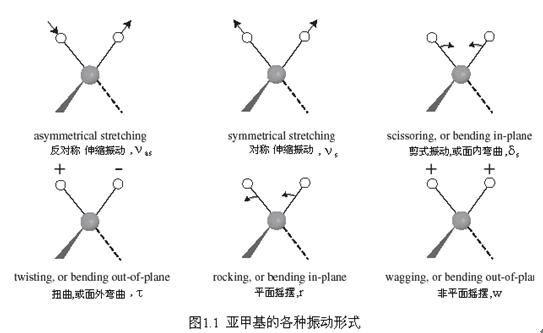
\includegraphics[height=1.in,width=2.in,viewport=0 20 420 250,clip]{Figures/RF_vir.jpg}
\caption{\small \textrm{Schematic example of vibration model of dimethyl.}}%
\label{virbration_model}
\end{figure} 
\textcolor{red}{简谐振动不表示某个原子的振动,表示整个体系所有原子参与的振动。这种体系中所有原子一起参加的共同振动常称为振动模}
}

\frame
{
	\frametitle{一维单原子链}
\begin{figure}[h!]
\centering
%\hspace*{-10pt}
\vspace*{-0.25in}
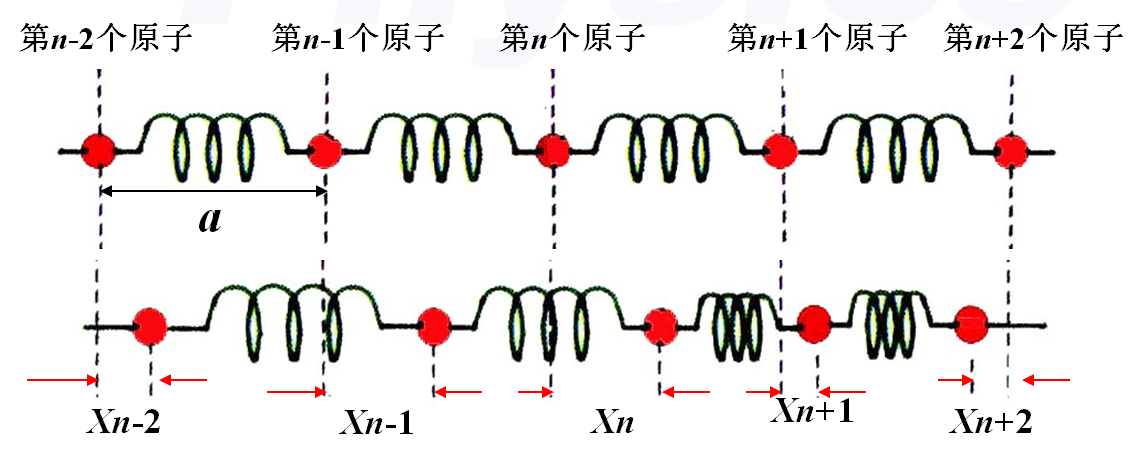
\includegraphics[height=1.0in,width=2.8in,viewport=0 0 1400 500,clip]{Figures/virbration.png}
\caption{\small \textrm{Schematic example of vibration of 1D-atomic chain.}}%
\label{virbration}
\end{figure} 
单原子链可以视为最简单的晶格,平衡时相邻原子距离为$\mathbf{a}$,原子限制在沿链方向运动,偏离格点位置用$\cdots,\mathbf{X}_{n-1},\mathbf{X}_{n},\mathbf{X}_{n+1},\cdots$,原子的振动可以表示为
\begin{displaymath}
	\mu_{nq}=A\mathrm{e}^{\mathrm{i}(\omega t-qx)}
\end{displaymath}
其中振幅$A$是常数,$\omega$是圆频率,$q=\tfrac{2\pi}{\lambda}$是波数,$\lambda$是波长\\
\textcolor{blue}{根据量子理论,每种简谐振动的能量是量子化的,可以用声子表示}
\begin{displaymath}
	\varepsilon_{nq}=\left( n+\frac12 \right)\hbar\omega_q
\end{displaymath}
}

\frame
{
	\frametitle{双原子链与光学支和声学支}
\begin{figure}[h!]
\centering
%\hspace*{-10pt}
\vspace*{-0.25in}
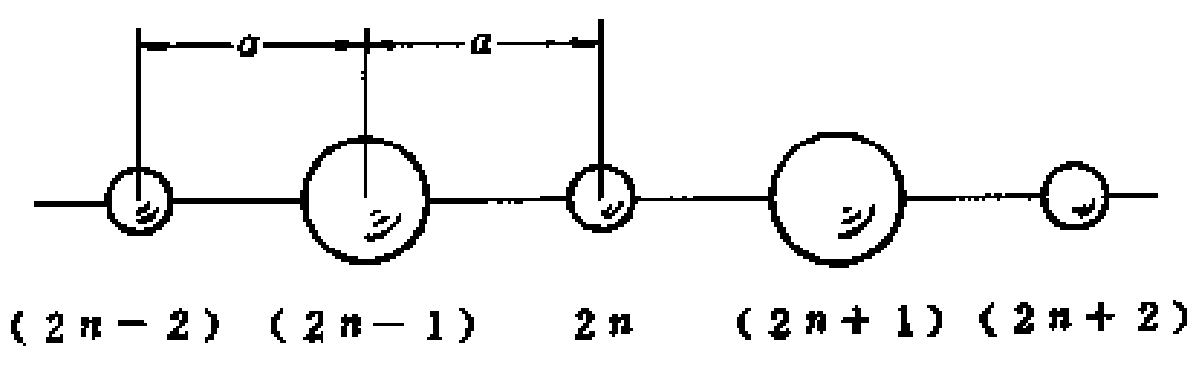
\includegraphics[height=0.7in,width=2.6in,viewport=0 0 1400 400,clip]{Figures/virbration-2.png}
\caption{\small \textrm{Schematic example of vibration of 1D-diatomic chain.}}%
\label{virbration-2D}
\end{figure} 
一维双原子链是最简单的复式晶格,平衡时相邻原子间距为$\mathbf{a}$,每个原胞含有两个不同原子\textrm{P}和\textrm{Q}质量分别是$m$和$M$,原子现在在沿链方向运动,偏离位移用$\cdots,\mu_{2n},\mu_{2n+1},\cdots$\\原子的运动方程
\begin{displaymath}
	\begin{aligned}
		&\mbox{\textrm{P}原子:~}m\ddot{\mu}_{2n}=-\beta(2\mu_{2n}-\mu_{2n+1}-\mu_{2n-1})\\
		&\mbox{\textrm{Q}原子:~}M\ddot{\mu}_{2n+1}=-\beta(2\mu_{2n+1}-\mu_{2n+2}-\mu_{2n})
	\end{aligned}
\end{displaymath}
可得关于振动频率$\omega$的两组解
\begin{displaymath}
	\omega^2\left.
	\begin{aligned}
		&\nearrow\omega_+^2\\
		&\searrow\omega_-^2
	\end{aligned}\right\}
	=\beta\frac{m+M}{mM}\left\{ 1\pm\left[ 1-\frac{4mM}{(m+M)^2}\sin^2aq \right]^{1/2} \right\}
\end{displaymath}
}

\frame
{
	\frametitle{光学支和声学支的长波极限}
\begin{figure}[h!]
\begin{minipage}[t]{0.3\linewidth}
\centering
\vspace*{-0.3in}
%\hspace*{-10pt}
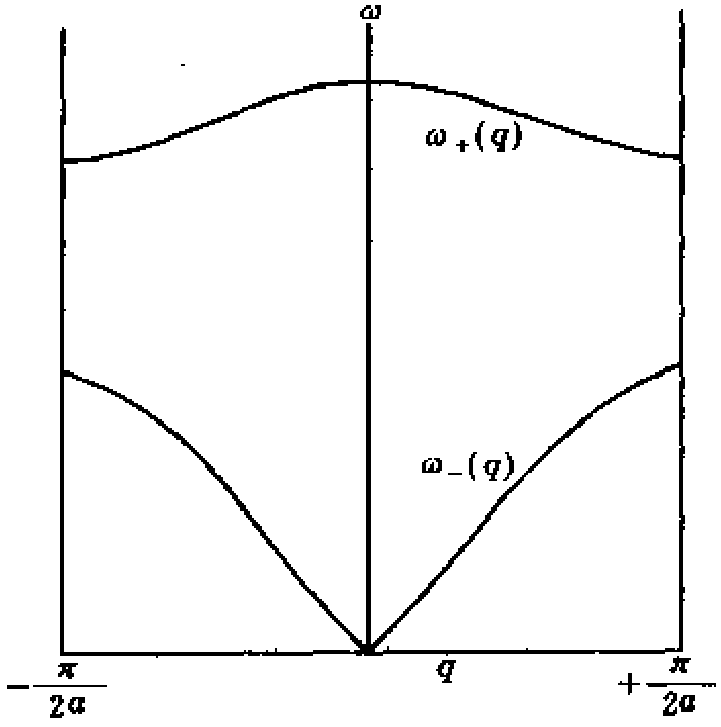
\includegraphics[height=1.in,width=1.in,viewport=0 0 700 800,clip]{Figures/Optic-Acous.png}
\label{optic_acous}
\end{minipage}
\hfill
\begin{minipage}[t]{0.67\linewidth}
%\vspace*{-0.3in}
	\begin{itemize}
		\item \textcolor{blue}{光学支}:~属于频率$\omega_+$的晶格简谐振动
		\item \textcolor{blue}{声学支}:~属于频率$\omega_-$的晶格简谐振动
	\end{itemize}
\end{minipage}
\caption{\small \textrm{The acoustic branch and optical branch.}}%
\end{figure} 
声学支的长波极限($q\rightarrow0$):
\begin{displaymath}
	\omega_-\approx a\sqrt{\frac{2\beta}{m+M}}q\quad\mbox{\textcolor{blue}{一维链看成连续介质的弹性波}}
\end{displaymath}
光学支的长波极限($q\rightarrow0$):
\begin{displaymath}
	\omega_+\approx a\sqrt{\frac{2\beta}{\left( \frac{mM}{m+M} \right)}}\quad\mbox{\textcolor{blue}{两种原子具有相反的相位,质心保持不动}}
\end{displaymath}
}

\frame
{
	\frametitle{经典三维振动模式}
			位于$\mathbf{R}_I(t)$的原子核运动的经典力学描述
			\begin{displaymath}
				M_I\frac{\partial^2\mathbf{R}_I}{\partial t^2}=\vec F_I(\mathbf{R})=-\frac{\partial}{\partial\mathbf{R}_I}E(\mathbf{R})
			\end{displaymath}
			晶格平衡位置$\{\mathbf{R}_I^0\}=\mathbf R^0$由原子核受力平衡确定
			\begin{displaymath}
				\vec F_I(\mathbf R^0)=0
			\end{displaymath}
			\textcolor{blue}{对平衡位置偏移的受力方程为}
			\begin{displaymath}
				C_{I,\alpha;J,\beta}=\frac{\partial^2E(\mathbf{R})}{\partial\mathbf{R}_{I,\alpha}\partial\mathbf{R}_{J,\beta}}
			\end{displaymath}
			其中$\alpha,\beta\cdots$是\textrm{cartesian}坐标

			\textcolor{blue}{谐振子近似下},频率为$\omega$的谐振模式下,晶格对平移位置的偏移为
			\begin{displaymath}
				\mathbf{u}_I(t)=\mathbf{R}_I(t)-\mathbf{R}_I^0\equiv\mathbf{u}_I\mathrm{e}^{\mathrm{i}\omega t}
			\end{displaymath}
			对位于$I$的原子核(质量为$M_I$),有
			\begin{displaymath}
				-\omega^2M_Iu_{I\alpha}=-\sum_{J\beta}C_{I,\alpha;J\beta}u_{J\beta}
			\end{displaymath}
			因此振动频率$\omega$,由经典谐振方程确定
			\begin{displaymath}
				\det\left|\frac1{\sqrt{M_IM_J}}C_{I,\alpha;J\beta}-\omega^2\right|=0
			\end{displaymath}
}

\frame
{
	\frametitle{晶格振动模式(冻声子方法)}
	对于周期性的晶格振动,根据\textrm{Bl\"och~}定理,振动引起的位置偏移
			\begin{displaymath}
				\mathbf{u}_s(\vec T_n)\equiv\mathbf{R}_s(\vec T_n)-\mathbf{R}_s^0(\vec T_n)=\mathrm{e}^{\mathrm{i}\vec k\cdot\vec T_n}\mathbf{u}_s(\vec k)
			\end{displaymath}
			由此得谐振方程
			\begin{displaymath}
				\det\left|\frac1{\sqrt{M_sM_{s^{\prime}}}}C_{s,\alpha;s^{\prime}\alpha^{\prime}}-\omega_{i\vec k}^2\right|=0
			\end{displaymath}
			这里原子标记$s=1,S$,对应的谐振模式$i=1,3S$

			每个$\vec k$的约化力常数矩阵可表示为
			\begin{displaymath}
				\begin{aligned}
				C_{s,\alpha;s^{\prime}\alpha^{\prime}}(\vec k)=&\sum_{\vec T_n}\mathrm{e}^{\mathrm{i}\vec k\cdot\vec T_n}\frac{\partial^2 E(\mathbf{R})}{\partial\mathbf{R}_{s,\alpha}(0)\partial\mathbf{R}_{s^{\prime},\alpha^{\prime}}(\vec T_n)}\\
				=&\frac{\partial^2E(\mathbf{R})}{\partial\mathbf{u}_{s,\alpha}(\vec k)\partial\mathbf{u}_{s^{\prime},\alpha^{\prime}}(\vec k)} 
				\end{aligned}
			\end{displaymath}
}

\frame
{
	\frametitle{声子与密度响应函数}
	谐振的力常数是能量的两阶导数,因此最初由响应函数计算声子时,即采用两阶微扰理论

	对于随参数$\lambda_i$变化的外势$V_{ext}(\vec r)$的响应中包含一般表达式
	\begin{displaymath}
		\begin{aligned}
			\frac{\partial E}{\partial\lambda_i}=&\frac{\partial E_{\mathrm{ion}}}{\partial\lambda_i}+\int\frac{\partial V_{ext}(\vec r)}{\partial\lambda_i}n(\vec r)\mathrm{d}\vec r\quad\mbox{\textcolor{red}{即\textrm{Hellmann-Feynman}力}}\\
			\frac{\partial^2E}{\partial\lambda_i\partial\lambda_j}=&\frac{\partial^2E_{\mathrm{ion}}}{\partial\lambda_i\partial\lambda_j}+\int\frac{\partial^2V_{ext}(\vec r)}{\partial\lambda_i\partial\lambda_j}n(\vec r)\mathrm{d}\vec r+\underline{\int\frac{\partial n(\vec r)}{\partial\lambda_i}\frac{\partial V_{ext}(\vec r)}{\partial\lambda_j}\mathrm{d}\vec r}
		\end{aligned}
	\end{displaymath}
	其中
	\begin{displaymath}
		\begin{aligned}
	\int\frac{\partial n(\vec r)}{\partial\lambda_i}\frac{\partial V_{ext}(\vec r)}{\partial\lambda_j}\mathrm{d}\vec r=&\int\frac{\partial V_{ext}(\vec r^{\prime})}{\partial\lambda_i}\frac{\partial n(\vec r)}{\partial V_{ext}(\vec r^{\prime})}\frac{\partial V_{ext}(\vec r)}{\partial\lambda_j}\mathrm{d}\vec r\mathrm{d}\vec r^{\prime}\\
		=&\int\frac{\partial V_{ext}(\vec r^{\prime})}{\partial\lambda_i}\chi(\vec r,\vec r^{\prime})\frac{\partial V_{ext}(\vec r)}{\partial\lambda_j}\mathrm{d}\vec r\mathrm{d}\vec r^{\prime}
		\end{aligned}
	\end{displaymath}
	这里\textcolor{red}{$\chi$是密度响应函数}
}

\frame
{
	\frametitle{密度响应函数与\textrm{Green's function}表示}
	密度响应函数$\chi$可以在$\vec r$空间或$\vec q$空间表示
	\begin{displaymath}
		\chi(\vec r,\vec r^{\prime})=\frac{\delta n(\vec r)}{\delta V_{ext}(\vec r^{\prime})}\qquad\chi(\vec q,\vec q^{\prime})=\frac{\delta n(\vec q)}{\delta V_{ext}(\vec q^{\prime})}
	\end{displaymath}
	响应函数可表示为
	\begin{displaymath}
		\chi=\frac{\delta n}{\delta V_{\mathrm{eff}}}\frac{\delta V_{\mathrm{eff}}}{\delta V_{ext}}=\chi^0\left[1+\frac{\delta V_{int}}{\delta n}\frac{\delta n}{\delta V_{ext}}\right]=\chi^0[1+K\chi]
	\end{displaymath}
	其中$\chi^0$是无相互作用的响应函数,$K$是\textrm{kernel~}函数
	\begin{displaymath}
		\chi_n^0(\vec r,\vec r^{\prime})=\frac{\delta n(\vec r)}{\delta V_{\mathrm{eff}}(\vec r^{\prime})}=2\sum_{i=1}^{\mathrm{occ}}\sum_j^{\mathrm{empty}}\frac{\psi_i^{\ast}(\vec r)\psi_j(\vec r)\psi_j^{\ast}(\vec r^{\prime})\psi_i(\vec r^{\prime})}{\varepsilon_i-\varepsilon_j}
	\end{displaymath}
	可用\textrm{Green's function}表示
	\begin{displaymath}
		\chi_n^0(\vec r,\vec r^{\prime})=\sum_{i=1}^{\mathrm{occ}}\psi_i^{\ast}(\vec r)G_0^i(\vec r,\vec r^{\prime})\psi_i(\vec r^{\prime})\qquad G_0^i(\vec r,\vec r^{\prime})=\sum_{j\neq i}^{\infty}\frac{\psi_j(\vec r)\psi_j^{\ast}(\vec r^{\prime})}{\varepsilon_i-\varepsilon_j}
	\end{displaymath}
}

\frame
{
	\frametitle{密度响应函数的$\vec q$空间表示}
	注意到$\vec r$空间电荷密度变化
	\begin{displaymath}
		\Delta n(\vec r)=\sum_{i=1}^{\mathrm{occ}}\sum_j^{\mathrm{empty}}\psi_i^{\ast}(\vec r)\psi_j(\vec r)\frac{\langle\psi_j|\Delta V_{\mathrm{eff}}|\psi_i\rangle}{\varepsilon_i-\varepsilon_j}+\mathrm{c.c.}
	\end{displaymath}
	因此在$\vec q$空间表示中,$\Delta V_{\mathrm{eff}}(\vec r)=\Delta V_{\mathrm{eff}}\mathrm{e}^{\mathrm{i}\vec q\cdot\vec r}$,$n(\vec q^{\prime})=\int\mathrm{d}\vec rn(\vec r)\mathrm{e}^{\mathrm{i}\vec q\cdot\vec r}$,\\可有
	\begin{displaymath}
		\chi_n^0(\vec q,\vec q^{\prime})=\frac{\delta n(\vec q^{\prime})}{\delta V_{\mathrm{eff}}(\vec q)}=2\sum_{i=1}^{\mathrm{occ}}\sum_j^{\mathrm{empty}}\frac{M_{ij}^{\ast}(\vec q)M_{ij}(\vec q^{\prime})}{\varepsilon_i-\varepsilon_j}
	\end{displaymath}
	这里$M_{ij}(\vec q)=\langle\psi_i|\mathrm{e}^{\mathrm{i}\vec q\cdot\vec r}|\psi_j\rangle$\\
	\vspace{10pt}
	\textcolor{blue}{显然对于周期体系,$\chi_n^0$在$\vec q$空间表示更方便}
	
	对于均匀电子气,只有$\vec q=\vec q^{\prime}$,$\chi_n^0(\vec q,\vec q^{\prime})\neq0$
}

\frame
{
	\frametitle{密度响应函数与声子}
	\textrm{kernel~}函数$K$的表达式
	\begin{displaymath}
		K(\vec q,\vec q^{\prime})=\frac{\delta V_{ini}(\vec q)}{\delta n(\vec q^{\prime})}=\frac{4\pi}{q^2}\delta_{\vec q,\vec q^{\prime}}+\frac{\delta^2 E_{\mathrm{XC}}[n]}{\delta n(\vec q)\delta n(\vec q^{\prime})}\equiv V_C(q)\delta_{\vec q,\vec q^{\prime}}+f_{\mathrm{XC}}(\vec q,\vec q^{\prime})
	\end{displaymath}
	\textcolor{red}{注意}:~当$f_\mathrm{XC}=0$即无规相近似(\textrm{random phase approximation, RPA})\\
	由此可得
	\begin{displaymath}
		\chi=\chi^0[1-\chi^0K]^{-1}\qquad\chi^{-1}=[\chi^0]^{-1}-K
	\end{displaymath}
介电函数也可以用响应函数表示
	\begin{displaymath}
		\epsilon^{-1}=1+V_\mathrm{C}\chi
	\end{displaymath}
	因此对于\textit{sp}-型金属,$\chi$可以用均匀电子气模型表示(\textrm{Lindhard}介电函数$\epsilon^{-1}(|\vec q|)$),但是对于一般材料介电函数$\epsilon^{-1}(\vec q,\vec q^{\prime})$变成很大的矩阵$\epsilon_{\vec G\vec G^{\prime}}^{-1}(\vec k)$,计算非常困难
}

\frame
{
	\frametitle{\textrm{Green's function~}方法}
	\begin{itemize}
		\item 利用标准微扰理论,计算介电函数矩阵倒数$\epsilon_{\vec G\vec G^{\prime}}^{-1}(\vec k)$虽然\textcolor{blue}{能给出全部可能微扰的响应},但涉及\textcolor{red}{对全部未占据态的求和},计算效率很低
		\item 近年来发展的密度泛函微扰理论\textrm{(density functional perturbation theory, DFPT)}只关注\textcolor{blue}{特定微扰的响应},因此\textcolor{red}{计算中只需要对占据态的求和},大大提高计算效率
			\begin{enumerate}
				\item 响应函数的自洽方程用波函数改变表示\\
					电荷密度的一阶改变
					\begin{displaymath}
						\Delta n(\vec r)=2\mathrm{Re}\sum_{\i=1}^N\psi_i(\vec r)\Delta\psi_i(\vec r)
					\end{displaymath}
					其中$\Delta\psi_i(\vec r)$由一阶微扰计算
					\begin{displaymath}
						(H_{\mathrm{KS}}-\varepsilon_i)|\Delta\psi_i\rangle=-(\Delta V_{\mathrm{KS}}-\Delta\varepsilon_i)|\psi_i\rangle
					\end{displaymath}
			\end{enumerate}
	\end{itemize}
}

\frame
{
	\frametitle{\textrm{Green's function~}方法}
	$\Delta\varepsilon_i=\langle\psi_i|\Delta V_{\mathrm{KS}}|\psi_i\rangle$,因此有效势的改变可用电荷密度的变化表示
	\begin{displaymath}
		\begin{aligned}
			\Delta V_{\mathrm{KS}}(\vec r)=&\Delta V_{ext}(\vec r)+e^2\int\mathrm{d}\vec r^{\prime}\frac{\Delta n(\vec r^{\prime})}{|\vec r-\vec r^{\prime}|}+\int\mathrm{d}\vec r^{\prime}\frac{\mathrm{d}V_{\mathrm{XC}}(\vec r)}{\mathrm{d}n(\vec r^{\prime})}\Delta n(\vec r^{\prime})\\
			\equiv&\Delta V_{ext}(\vec r)+\int\mathrm{d}r^{\prime}K(\vec r,\vec r^{\prime})\Delta n(\vec r)
		\end{aligned}
	\end{displaymath}
	根据\textrm{kernel~}函数的定义,其中交换-相关部分贡献的一阶近似为$f_{\mathrm{XC}}(\vec r,\vec r^{\prime})=\tfrac{\mathrm{d}V_{\mathrm{XC}}(\vec r)}{\mathrm{d}n(\vec r^{\prime})}$
	\begin{itemize}
		\item \textcolor{blue}{根据标准微扰理论,由于电荷密度的变化遍及全部占据态($i\leqslant N$)和未占据态($j>N$)求和,因此计算效率不高}
		\item \textcolor{red}{更有效的办法是将密度和有效势的变化$\Delta n$、$\Delta V_{\mathrm{KS}}$看做为外势变化$\Delta V_{ext}$的自洽响应}\\
定义投影算符
\begin{displaymath}
%	\begin{aligned}
		\hat P_{\mathrm{occ}}=\sum_{i=1}^N|\psi_i\rangle\langle\psi_i|\quad\mbox{(占据态)}\quad%\\
		\hat P_{\mathrm{empty}}=1-\hat P_{\mathrm{occ}}\quad\mbox{(未占据态)}
%	\end{aligned}
\end{displaymath}
	\end{itemize}
}

\frame
{
	\frametitle{\textrm{Green's function~}方法}
因此对于占据轨道的修正
					\begin{displaymath}
						(H_{\mathrm{KS}}-\varepsilon_i)|\Delta\psi_i\rangle=-\hat P_{\mathrm{empty}}\Delta V_{\mathrm{KS}}|\psi_i\rangle
					\end{displaymath}
					在\textrm{DFPT}框架下即可用上述方程的迭代构成

					\begin{enumerate}
						\setcounter{enumi}{1}
						\item 响应函数的变分表达
							\begin{displaymath}
								\begin{aligned}
									E^{(2)}[V_{ext},n]=&E[V_{ext}^0,n^0]+\int\mathrm{d}\vec rn^0(\mathrm{d}\vec r)\Delta V_{ext}(\vec r)\\
									+&\frac12\int\mathrm{d}\vec r\mathrm{d}\vec r^{\prime}\left[ \frac{\delta^2E}{\delta V_{ext}(\vec r)\Delta n(\vec r^{\prime})} \right]\Delta V_{ext}(\vec r)\Delta n(\vec r^{\prime})\\
									+&\frac12\int\mathrm{d}\vec r\mathrm{d}\vec r^{\prime}\left[ \frac{\delta^2E}{\delta n(\vec r)\delta n(\vec r^{\prime})} \right]\Delta n(\vec r)\Delta n(\vec r^{\prime})
								\end{aligned}
							\end{displaymath}
					\end{enumerate}
}

\frame
{
	\frametitle{\textrm{Green's function~}方法}
	用波函数作为基本变量
							\begin{displaymath}
								\begin{aligned}
									E^{(2)}[V_{ext},\psi_i]=&E[V_{ext}^0,\psi_i^0]\\
									+&\frac12\sum_i\int\mathrm{d}\vec r\mathrm{d}\vec r^{\prime}\left[ \frac{\delta^2E}{\delta V_{ext}(\vec r)\delta\psi_i(\vec r^{\prime})} \right]\Delta V_{ext}(\vec r)\Delta\psi_i(\vec r^{\prime})\\
									+&\frac12\sum_{ij}\int\mathrm{d}\vec r\mathrm{d}\vec r^{\prime}\left[ \frac{\delta^2E}{\delta\psi_i(\vec r)\delta\psi_j(\vec r^{\prime})} \right]\Delta\psi_i(\vec r)\Delta\psi_i(\vec r^{\prime})
								\end{aligned}
							\end{displaymath}
							其中
							\begin{displaymath}
								\begin{aligned}
									\frac{\delta^2E}{\delta V_{ext}(\vec r)\delta\psi_i(\vec r^{\prime})}=&\psi_i^0(\vec r)\delta(\vec r-\vec r^{\prime})\\
									\frac{\delta^2E}{\delta V_{ext}(\vec r)\delta\psi_i(\vec r^{\prime})}=&H_{\mathrm{KS}}^0(\vec r,\vec r^{\prime})+K(\vec r,\vec r^{\prime})\Delta\psi_i(\vec r)\Delta\psi_j(\vec r^{\prime})\Delta\psi_i(\vec r)\Delta\psi_j(\vec r^{\prime})
								\end{aligned}
							\end{displaymath}

}

\frame
{
	\frametitle{\textrm{Green's function~}方法}
	由约束条件
	\begin{displaymath}
		\langle\psi_i^0+\Delta\psi_i|\psi_j^0+\Delta\psi_j\rangle=\delta_{ij}
	\end{displaymath}
	可有
	\begin{displaymath}
		H_{\mathrm{KS}}^0\Delta\psi_i-\sum_j\Lambda_{ij}\Delta\psi_j=-(\Delta V_{\mathrm{eff}}-\varepsilon_i)\psi_i+\sum_j\Lambda_{ij}\Delta\psi_j
	\end{displaymath}
	\begin{enumerate}
		\setcounter{enumi}{2}
	\item 对于周期体系,由声子波矢$\vec k_p$产生的微扰,用\textrm{DFPT}可以极大简化
		\begin{displaymath}
			\hspace*{-37pt}
			\begin{aligned}
					\Delta V_{ext}(\vec r)=\Delta v_{ext}^{\vec k_p}(\vec r)\mathrm{e}^{\mathrm{i}\vec k_p\cdot\vec r}=&\sum_{\vec T}\frac{V_s[\vec r-\mathbf{R}_s(\vec T)]}{\partial\mathbf{R}_s(\vec T)}\mathrm{e}^{-\mathrm{i}\vec k_p\cdot(\vec r-\mathbf{R}_s(\vec T))}\mathbf{u}_s(\vec k_p)\mathrm{e}^{\mathrm{i}\vec k_p\cdot\vec r}\\
				\Delta V_{\mathrm{KS}}(\vec r)=&\Delta v_{\mathrm{KS}}^{\vec k_p}(\vec r)\mathrm{e}^{\mathrm{i}\vec k_p\cdot\vec r}\\
				\Delta n(\vec r)=&\Delta n^{\vec k_p}(\vec r)\mathrm{e}^{\mathrm{i}\vec k_p\cdot\vec r}
			\end{aligned}
		\end{displaymath}
	\end{enumerate}
}

\frame
{
	\frametitle{\textrm{Green's function~}方法}
	由此引起的电子波矢$\vec k_e$的改变为$\vec k_e+\vec k_p$
	\begin{displaymath}
		(H_{\mathrm{KS}}^{\vec k_e}-\varepsilon_i^{\vec k_e})|\Delta\psi_i^{\vec k_e+\vec k_p}\rangle=-[1-\hat P_{\mathrm{occ}}^{\vec k_e+\vec k_p}]\Delta V_{\mathrm{KS}}^{\vec k_p}|\psi_i^{\vec k_e}\rangle
	\end{displaymath}
	密度的线性响应
	\begin{displaymath}
		\Delta n^{\vec k_p}(\vec r)=2\sum_{\vec k_e,i}u_{\vec k_e,i}^{\ast}(\vec r)\Delta u_{(\vec k_e+\vec k_{p}),i}(\vec r)
	\end{displaymath}
	\textrm{Kohn-Sham~}势
	\begin{displaymath}
		\Delta v_{\mathrm{KS}}^{\vec k_p}(\vec r)=\Delta v_{ext}^{\vec k_p}(\vec r)+\int\mathrm{d}\vec r^{\prime}\left[ \frac1{|\vec r-\vec r^{\prime}|}+f_{\mathrm{XC}}(\vec r,\vec r^{\prime}) \right]\Delta n^{\vec k_p}(\vec r)
	\end{displaymath}

}

\frame{
	\frametitle{介电响应函数}
	\begin{itemize}
		\item 由于\textrm{Coulomb~}作用的长程特征,电场的存在对物理性质(包括介电函数、有效电荷和压电常数等)会有明显影响
		\item 对于周期体系,匀强电场产生外势$V_{ext}(\vec r)=\vec E\cdot\vec r$在长波极限下($\vec q=0$)的\textrm{Hamiltonian~}是病态的,必须借助微扰理论
		\item 根据微扰理论,对外加电场响应的\textrm{Hamiltonian~}矩阵元可以表示为
			\begin{displaymath}
				\langle\psi_i|\vec r|\psi_j\rangle=\frac{\langle\psi_i|[H,\vec r]|\psi_j\rangle}{\varepsilon_i-\varepsilon_j}\quad i\neq j
			\end{displaymath}
			\begin{enumerate}
				\item 当电子感受到的势是局域势时,对易关系可简化为
					\begin{displaymath}
						[H,\vec r]=-\frac{\hbar^2}{m_e}\frac{\partial}{\partial\vec r}=\mathrm{i}\frac{\hbar}{m_e}\vec p
					\end{displaymath}
				\item 对于非局域势的情况
					\begin{displaymath}
						[H,\vec r]=\mathrm{i}\frac{\hbar}{m_e}\vec p+[\delta V_{nl},\vec r]
					\end{displaymath}
			\end{enumerate}
	\end{itemize}
}

\section{电-声耦合}
\frame
{
	\frametitle{电-声耦合}
	电子-声子的来源:~\textcolor{blue}{$C_{ii^{\prime}}$的非对角元部分}
	\begin{itemize}
		\item $C_{ii^{\prime}}$的非对角元部分描述了\textcolor{red}{原子核运动(振动)引起电子在不同态间跃迁}
		\item $C_{ii^{\prime}}$的非对角元部分主要来自$A_{ii^{\prime}}$
			\begin{enumerate}
				\item 电子波函数$\Psi_i(\{\mathbf{r}\}:\{\mathbf{R}\})$对原子核位置$\{\mathbf{Rj}\}$的梯度
				\item 梯度算符对声子波函数$\chi_{si}(\{\mathbf{R}\})$的贡献
			\end{enumerate}
		\item 电子在态$i\rightarrow i^{\prime}$跃迁将会激发或吸收一个声子
	\end{itemize}
	线性近似下有
	\begin{displaymath}
		\hspace*{-15pt}
		\langle\Psi_i(\{\mathbf{r}\}:\{\mathbf{R}\})|\nabla_J|\Psi_i^{\prime}(\{\mathbf{r}\}:\{\mathbf{R}\})\rangle=\frac{\langle\Psi_i(\{\mathbf{r}\}:\{\mathbf{R}\})|\tfrac{\nabla_V}{\nabla_{\mathbf{R}_J}}|\Psi_{i^{\prime}}(\{\mathbf{r}\}:\{\mathbf{R}\})\rangle}{E_{i^{\prime}}(\{\mathbf{R}\})-E_i(\{\mathbf{R}\})}
	\end{displaymath}
}

\frame
{
	\frametitle{电-声耦合}
	\begin{itemize}
		\item 电-声耦合在固体输运和超导理论中有着重要的作用
		\item 根据微扰理论,当电子由始态$i\vec k$被散射到终态$j\vec k+\vec q$时,将会吸收或发射波矢$\nu\vec q$的声子(振动频率为$\omega$),其矩阵元可以表示为
			\begin{displaymath}
				g_{i\vec k;j\vec k+\vec q}(\nu)=\frac1{\sqrt{2M\omega_{\nu\vec q}}}\langle i\vec k|\Delta V_{\nu\vec q}|j\vec k+\vec q\rangle
			\end{displaymath}
			其中$M$是约化质量(与振动模式有关),$1/\sqrt{(2M\omega_{\nu\vec q})}$是声子的零点振幅
		\item 在微扰理论中,由原胞中原子偏移引入的势$\Delta V$近似到一阶
			\begin{displaymath}
				\Delta V_{v\vec q}=\frac{\partial V}{\partial u_{\nu\vec q}}=\sum{I\alpha}X_{\nu\vec q}(I\alpha)\frac{\partial V}{\partial u_{I\alpha}} 
			\end{displaymath}
			这里$u_{\nu\vec q}$是声子正则坐标,$X_{\nu\vec q}(I\alpha)$是动力学矩阵的本征矢,可用$\alpha$位置的原子核$I$偏移$u_{I\alpha}$表示
	\end{itemize}
}

\frame
{
	\frametitle{电-声耦合的微扰理论}
	\begin{itemize}
		\item 对于\textrm{Fermi~}面散射,对声学支$\nu$($\nu=1,2,\cdots,3S$)的耦合可表示为
			\begin{displaymath}
				\lambda_{nu}=\frac2{N(0)}\sum_{\vec q}\frac1{\omega_{\nu\vec q}}\sum_{ij\vec k}|g_{i\vec k;j\vec k+\vec q}(\nu)|^2\delta(\varepsilon_{i\vec k})\delta(\varepsilon_{j\vec k+\vec q}-\varepsilon_{i\vec k}-\omega_{\nu\vec q})
			\end{displaymath}
			这里$N(0)$是\textrm{Fermi~}能级的自旋态密度,$\omega_{\nu\vec q}$是波矢为$\vec q$的声子$\nu$的频率
	\end{itemize}
}

\appendix
%------------------------------------------------------------------------Reference----------------------------------------------------------------------------------------------
%\begin{thebibliography}{99}
%-----------------------------------------------------------------------------------------------------------------------------------------------------------------------%
%\frame
%{
%\frametitle{主要参考文献}
%{\small
%\bibitem{Singh_Book}\textrm{D. J. Singh. \textit{Plane Wave, PseudoPotential and the LAPW method} (Kluwer Academic, Boston,USA, 1994)}					%
%  \nocite{*}																				%
%}
%}
%\end{thebibliography}
\begin{thebibliography}{99}
\frame
{
\frametitle{主要参考文献}
{\small
	\bibitem{Huang_Han}黄昆\:原著、韩汝琦\:改编, {\textit{固体物理学}}\:高等教育出版社, 北京, 1988
	\bibitem{Huang_Han}阎守胜, {\textit{固体物理基础}}\:北京大学出版社, 北京, 2000
	\bibitem{Grosso_Parravicini}\textrm{Giuseppe Grosso and Giuseppe Pastori Parravicini, {\textit{Solid State Physics}} (Academic Press, Cambridge, U.K., 2000)}
	\bibitem{Elect_Stru}\textrm{Richard. M. Martin. \textit{Electronic Structure: Basic Theory and Practical Methods} (Cambridge University Press, Cambridge, England, 2004)}
%	\bibitem{PRL49-1691_1982}\textrm{P. Perdew, R. G. Parr, M. Levy and J. L. Balduz, Jr., \textit{Phys. Rev. Lett.} \textbf{49} (1982), 1691}
}
\nocite*{}
}
\end{thebibliography}

%{\small
%\phantomsection\addcontentsline{toc}{section}{Bibliography}	 %直接调用\addcontentsline命令可能导致超链指向不准确,一般需要在之前调用一次\phantomsection命令加以修正	%
%\bibliography{Myref}																			%
%\bibliographystyle{mybib}																		%
%  \nocite{*}																				%
%}
%-----------------------------------------------------------------------------------------------------------------------------------------------------------------------%


%-----------------------------------------------------------Beamer下不建议使用bib,因为涉及分页--------------------------------------------------------------------------%
%{\small
%\phantomsection\addcontentsline{toc}{section}{Bibliography}	 %直接调用\addcontentsline命令可能导致超链指向不准确,一般需要在之前调用一次\phantomsection命令加以修正	%
%\bibliography{Myref}																			%
%\bibliographystyle{mybib}																		%
%  \nocite{*}																				%
%}

%------------------------------------------------------------------------------------------------------------------------------------------------------------------------------%

%-------------------------------------------------------------------------Thanks------------------------------------------------------------------------------------------------
%\section{致谢}
%\frame
%{
%\frametitle{致$\quad$谢}
%\begin{itemize}
%    \setlength{\itemsep}{20pt}
%  \item 感谢本团队高兴誉、吴泉生、宋红州等各位老师参与的讨论
%  \item 感谢莫所长、宋主任以及软件中心各位老师和同事
%  \item 感谢王崇愚先生的帮助
%\end{itemize}
%}

\logo{}									%不显示logo
\frame
{
\vskip 60 pt
%\hskip 10pt \textcolor{blue}{\Huge 感谢答辩委员会各位老师\,\textrm{!}}\\
\vskip 35 pt
\hskip 60pt \textcolor{blue}{\Huge 谢谢大家\:!}
%\vskip 15 pt
%\hskip 40pt \textcolor{blue}{\Huge \textrm{for your attention\:!}}
}

%-------------------------------------------------------------------------------------------------------------------------------------------------------------------------------

\clearpage
%\end{CJK*}
\end{document}
